\section{Introduction to Ethereum}
\label{sec:eth-blockchain}
Open source blockchain networks like Ethereum and Bitcoin are software kits that allow you to create an economic system in software, replete with account management and a native unit of exchange that can be used to transfer funds between accounts. These native units of exchange are referred to as coins, tokens, or cryptocurrencies, but they are the same as tokens in any other system: they are a type of money that can only be used within that system to pay peers or run programs on the Ethereum network.
When you want to make one of these peer-to-peer networks accessible through a web browser, you need to use special software libraries such as Python Web3\footnote{\url{https://github.com/ethereum/web3.py}} which is utilized in this thesis to connect to the Ethereum network \cite[2]{dannen2017introducing}.

The fact that everyone in the world can interact with the blockchain, given you have internet access and an according device, such as a PC or mobile phone, is advantageous for a fixity storage such as presented in Chapter \ref{ch:fixity-storage}. Anyone is able to validate the integrity of an object with the right resources, e.g. the transaction in which an object's fixity information was originally stored. Picture a digital archive which releases multiple objects to the public and their respective fixity information on the blockchain, the community could then validate if the object in question is authentic. Pure trust, that an archive or its stewards did not tamper with the data in their care is therefore not needed anymore.
\section{About the Ethereum blockchain}
A block is a time unit that contains a specific amount of transactions. Transaction data is captured throughout that time period, and when the unit of time expires, the next block begins. The blockchain is a representation of the history of state changes in the Ethereum network \cite[43]{dannen2017introducing}.
The Ethereum network divides transactions and state changes into blocks, which are then hashed. Before the following canonical block may be added on top of it, each block is inspected and validated. Nodes on the network will no longer need to evaluate the trustworthiness of every single block in the Ethereum network's history, but only validate the most recent block in the chain. Therefore, it gets harder to tamper with past transactions with each block set on top of the blockchain. The blockchain is made up of all the blocks strung together, including the genesis block, which is the first block in the blockchain. The blockchain is also known as a distributed ledger or \acrlong{dlt} (\acrshort{dlt}). The term ledger is correct since the chain contains every transaction in the network's history, thereby turning it into a massive, well-balanced ledger \cite[55]{dannen2017introducing}. 
\section{Ethereum Virtual Machine (EVM)}
\label{sec:evm}
The physical manifestation of the \acrshort{evm} exist as a single entity sustained by thousands of connected computers running an Ethereum client\footnote{\url{https://ethereum.org/en/developers/docs/evm/}}.
In the Ethereum context, a virtual machine is a massive global computer made up of constituent nodes, which are themselves computers. In general, a virtual machine is a computer system that is emulated by another computer system. These emulations are based on the same computer architectures as the target of their emulation, but they usually reproduce that architecture on hardware other than that for which it was designed. Virtual machines can be built using hardware, software, or a combination of the two. It is both in the case of Ethereum. Rather than securing thousands of individual machines, Ethereum takes the approach of securing one massive state machine that can span the entire globe \cite[48]{dannen2017introducing}.

The \acrshort{evm} can run any computer program written in Solidity\footnote{\url{https://github.com/ethereum/solidity}}, the native programming language of the \acrshort{evm}. These programs will always create the same output, with the same underlying state changes, when given a specific input. As a result, Solidity programs are entirely deterministic and guaranteed to execute, as long as you pay enough for the transaction. Solidity programs are Turing complete in the sense that they can express all tasks that can be performed by computers. This means that every application executed on the platform is run by the entire dispersed network, every node \cite[50]{dannen2017introducing}.

The \acrshort{evm} is also a runtime environment for small programs that can be executed via a network, from the perspective of a software developer. Smart contracts are compiled into the \acrshort{evm}'s native language, the \acrshort{evm} bytecode. By using a client application like Truffle\footnote{\url{https://trufflesuite.com/}} or Geth\footnote{\url{https://geth.ethereum.org/}}, Solidity, a high-level language, is compiled into bytecode and posted onto the Ethereum network \cite[51]{dannen2017introducing}. I have decided to utilize Truffle for this thesis because of its fast and easy way to interact with the Ethereum network and its subnetworks.
\section{Smart Contracts}
Smart contracts, similar to the concept of classes in traditional object-oriented programming, are the building blocks of decentralized apps operating on the \acrshort{evm}. When developers talk about developing smart contracts, they usually mean writing applications in the Solidity programming language for execution on the Ethereum network \cite[10]{dannen2017introducing}.
In my thesis, the fixity storage is often referred to as \acrlong{dapp} (\acrshort{dapp}), which is an application built with several smart contracts. The smart contract implemented in this thesis is further described in Section \ref{sec:implementation}. 

\section{Persistence}\label{sec:persistence}
Decentralized storage systems, unlike centralized servers managed by a single corporation or organization, are made up of a peer-to-peer network of users that each hold a share or the whole amount of the data, resulting in a resilient file storage sharing system. All transactions in Ethereum are stored on the blockchain, a canonical history of state changes stored on every single Ethereum node \cite[12]{dannen2017introducing}. 
The chain is steadily growing and on March 19, 2022, the Ethereum chain is at 602.95 GB\footnote{\url{https://ycharts.com/indicators/ethereum_chain_full_sync_data_size}}, which every node on the network needs to be able to store. If the chain were to expand to large amounts of data (say 5TBs) it would not be feasible for all nodes to continue to run. Also, the cost of deploying this much data to the mainnet would be prohibitively expensive due to fees\footnote{\url{https://ethereum.org/en/developers/docs/storage/}}.
My proposed solution utilizing is pooled testing in order to mitigate the ever-increasing chain size of the Ethereum network by reducing the amount of transactions needed to operate the fixity storage. 

The blockchain, as a decentralized storage system also follows some rules, constrain and enforce relationships between entities. Motives to break or alter these relationships can be found in a wide range of industries, leading to bribery and corruption and making blockchain's trustless properties even more appealing to businesses than previous generations of software and networking. Shared read/write access generates considerable complexity. Depending on where the client's machine is located and regarding its internet speed, machines all over the world may experience variable latency, resulting in certain write operations arriving out of order. This becomes even more challenging when numerous parties are expected to share the blockchain equally \cite[20]{dannen2017introducing}. The Ethereum network solves this problem by nodes executing any code included within a block independently, this is possible due to the deterministic characteristic of the Solidity programming language. This method is not only highly parallelized, but also very redundant. Despite the significant redundancy, this is a reliable and efficient technique to balance a worldwide ledger \cite[50]{dannen2017introducing}.

Ethereum requires a persistence mechanism in order for a piece of data to last indefinitely. When executing a node, for example, the persistence method requires that the entire chain be considered. The chain continues to grow as new pieces of data are added to the end, requiring each node to reproduce all the embedded data. The term for this is "blockchain-based persistence." The problem with blockchain-based persistence is that the chain could grow to be far too large to maintain and retain all the data in a reasonable amount of time (e.g. many sources estimate the Internet to require over 40 Zetabytes of storage capacity). 

In addition, the blockchain must have some sort of incentive system for the participating nodes in the network to validate new blocks in the blockchain. Validating a block is a computational hard task which requires nodes to have a vast computing power which is used in a consensus mechanism called proof-of-work. In this consensus mechanism a cryptographic puzzle has to be solved, by the node which aims to validate a block, in order for a block to be seen as valid. The node which solves the puzzle and therefore presents the proof-of-work is rewarded with the so-called block-reward in form of \acrlong{eth} tokens. Ether is the name of the token, or cryptocurrency which is mainly used in the Ethereum ecosystem to pay for transactions or to fuel smart contracts. Ether can be publicly traded into other currencies such as EUR or USD.

For blockchain-based persistence, the incentive system includes a payment made to the miner, the payment varies with the amount of data which has to be included in a block\footnote{\url{https://ethereum.org/en/developers/docs/storage/}}.

\section{Test Networks}\label{sec:test-nets}
There are multiple independent networks implementing the Ethereum protocols, since the Ethereum source code is openly available everyone is able to set up an Ethereum network, which is often called a private fork. Networks can also be utilized as different Ethereum environments for development, testing or production use cases. The private key for an Ethereum account works across various Ethereum networks, but the transaction history or account balance is independent for each network, meaning you can not transfer funds from a test network to the mainnet and vice-versa. For testing purposes, I have utilized the Ropsten test network to deploy and interact with the fixity storage presented in Section \ref{ch:fixity-storage}. Interactions on the test network also requires you to have some funds in your wallet to pay for transactions, although the funds on the test network does not require you to gather them from exchanges for money. The \acrlong{eth} token for the Ropsten test network can be acquired through public faucets, where you receive some tokens after you have input your wallet address. Some faucets require you to have a Twitter account (e.g. \url{https://faucet.paradigm.xyz/}), with a certain amount of tweets and follower for bot protection and some faucets do have a large waiting queue for Ether tokens, in the case of \url{https://faucet.dimensions.network/} the waiting time can reach up to three days. Faucet are usually time gated, meaning that you could request \acrlong{eth} tokens only once per day. At small scale, this limitation is no problem for this thesis because persisting around ten pools on the blockchains require at max 0.002 \acrlong{eth} tokens. The one per day paradigm gets problematic for the experiment including 10,000 objects, which costs about 20 \acrlong{eth} tokens, which means I would have to request tokens for 20 days straight to perform one experiment on a real live environment such as the Ropsten test network. I have utilized each before presented faucet to gather funds for the experiment, my suggestion for future work is to use the following Ropsten test network faucet: \url{https://faucet.egorfine.com/}. This faucet does require you to either have an active social media account, neither does it implement a waiting queue.
There are multiple options to choose from for a testnet, from the most prominent networks presented at the official Ethereum documentation\footnote{\url{https://ethereum.org/en/developers/docs/networks/}} only the Ropsten test network implements the proof-of-work algorithm, which means it is the best representation of Ethereum to date, and for that reason I decided to utilize the Ropsten test network in my thesis.

\section{Gas and Fees}
\label{sec:costs}
Gas refers to the unit that measures the amount of computational effort required to execute specific operations on the Ethereum network, this property allows you to calculate the operation cost for the fixity storage without taking the price fluctuation of ETH into account. Since each Ethereum transaction requires computational resources to execute, each transaction requires a fee.
Gas fees are paid in \acrlong{eth} tokens. Gas prices are denoted in \acrlong{gwei}, which itself is a denomination of \acrshort{eth} - each \acrshort{gwei} is equal to 0.000000001 ETH. For example, instead of saying that your gas costs 0.000000001 \acrlong{eth}, you can say your gas costs 1 \acrlong{gwei}. The word "\acrlong{gwei}" itself means "giga-wei", and it is equal to 1,000,000,000 wei. Wei itself is the smallest unit of the \acrlong{eth} token\footnote{\url{https://ethdocs.org/en/latest/ether.html}}.

Miners are paid in \acrlong{eth} tokens for validating blocks, and also for running scripts on the network. The cost associated with electricity consumption of nodes running the Ethereum network is one of the factors that gives \acrlong{eth}, as a cryptocommodity, its intrinsic value—that is, someone paid real money to their electricity company to run their mining machine. Specialized mining rigs, which use arrays of graphics cards to increase their odds of solving the cryptographic puzzle in the proof-of-work mechanism, and therefore completing a block and collect the block-reward \cite[12]{dannen2017introducing}. 
Mining creates the consensus needed to make legitimate state changes in the distributed ledger, and miners are compensated for their contributions. This is how \acrlong{eth} tokens and Bitcoins are created \cite[57]{dannen2017introducing}. 
To ensure that the system is not clogged by meaningless spam contracts, there must be a fee associated with each instruction the \acrshort{evm} executes. An internal counter maintains the amount of the fees incurred each time an instruction is executed, which are then charged to the user. When a user initiates a \gls{transaction}, a tiny percentage of the user's fund is set aside to pay these fees \cite[58]{dannen2017introducing}. 

The costs are the driving factor of my thesis where I try to make as few transactions as possible to run a fixity storage on the Ethereum network. 
The fees are determined by the transaction's gas cost; gas is a unit of effort, not a subcurrency, therefore it cannot be held or hoarded. In computer words, it simply assesses how much work each step of a transaction will take. You need enough \acrlong{eth} tokens in your account to be able to pay for the transaction, or else it will get reverted. There is no need to buy gas individually because there is no gas token. Gas prices ensure that network computing time is adequately priced and varies with the time of the day, meaning the more traffic there is on the network the higher are the gas prices for transactions or smart contract calls \cite[59]{dannen2017introducing}.
The only person who suffers if you transmit a set of computationally difficult commands to the \acrshort{evm} is you, it has no bearing on the transactions of others. There is no method to jam the \acrlong{evm} without spending a significant amount of money in transaction fees. The gas price system serves as a de facto means of scalability. Miners have complete control over which transactions they will include in a block, depending on which transaction pays the highest fee rates, as well as the block gas limit. The block gas limit sets the maximum amount of processing and storage that can be done per block \cite[60]{dannen2017introducing}. 

\section{Transactions}\label{sec:tx-cost}
An Ethereum transaction refers to an action initiated by an externally-owned account, in other words an account managed by a human, not a contract. For example, if Bob sends Alice 1 \acrshort{evm}, Bob's account must be debited and Alice's must be credited. This state-changing action takes place within a transaction. It is a mechanism for an external account to provide the \acrshort{evm} instructions to do a task. To put it another way, it is a method for an external account to send a message to the system. A transaction in the \acrshort{evm} is a cryptographically signed data package storing a message, which tells the \acrshort{evm} to transfer tokens, create a new smart contract, interact with an existing one, or perform some calculation. Contract addresses, like users with external accounts, can be transaction recipients \cite[60]{dannen2017introducing}. 
\begin{figure}[t]
    \centering
    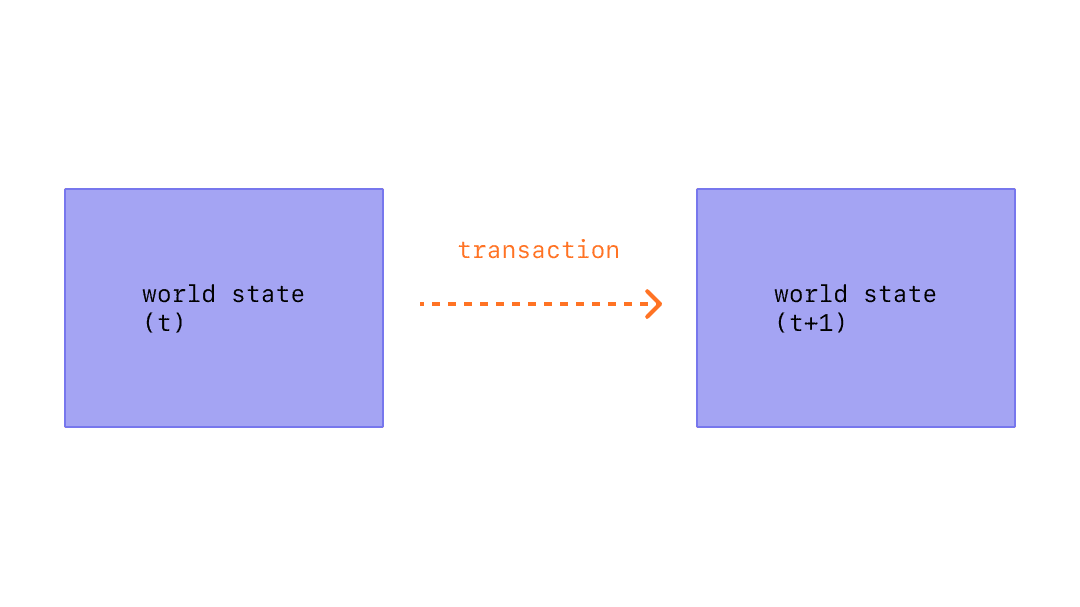
\includegraphics[width=0.5\textwidth]{eth_transaction.png}
    \caption{Illustration of an Ethereum transaction \url{https://ethereum.org/en/developers/docs/transactions/}}
\end{figure}
Transactions that affect the \acrshort{evm}s state must be broadcast to the entire network. A miner will execute the transaction and propagate the resulting state change to the rest of the network once any node broadcasts a request for a transaction to be conducted on the \acrshort{evm}\footnote{\url{https://ethereum.org/en/developers/docs/transactions/}}.
Transactions, which do not alter the global state are free of charged and are referred to as Calls. As seen in the source code in Listing \ref{lst:fixity-storage}, \textit{getPoolHash(uint32 poolId)} is marked with the keyword \textbf{view}, which means the function itself does not alter the state of the network. Contrary to the function \textit{setPoolHash(uin32 poolId, bytes32 poolHash)} which does alter the networks state and therefore generates cost for the fixity storage. In this thesis, writing actions on the blockchain are often referred to as Transactions; and reading actions are referred to as Calls.
Table \ref{table:gas-costs} presents the gas cost of the most relevant network operations used in this thesis according to the Ethereum yellow paper \cite[27]{wood2014ethereum}.
\begin{center}
    \begin{tabular}{ l l l }\label{table:gas-costs}
        Operation Name & Gas Cost & Description \\ 
        $codedeposit$ & 200 & gas cost per byte the compiled smart contract \\  
        $txcreate$ & 32000 & create a new smart contract  \\   
        $transaction$ & 21000 & base cost for a transaction \\
        $txdatazero$ & 4 & gas cost for every zero byte of the transaction data  \\   
        $txdatanonzero$ & 16 & gas cost for every non-zero byte of the transaction data  \\   
        $sset$ & 20000 & set a persistent variable for the first time in the contract \\
        $sreset$ & 2900 & the cost for updating a persistent variable 
    \end{tabular}
\end{center}

\section{Summary}
The learnings in this chapter is on how to interact with the Ethereum network, which tools to use and how the computational cost comes about. I have presented that it is important to prune all unnecessary transaction and storage data to mitigate the ever-increasing chain size of the Ethereum blockchain and reduce the cost for the user of the fixity storage presented in Chapter \ref{ch:fixity-storage}. 